%%This is a very basic article template.
%%There is just one section and two subsections.
\documentclass[a4paper]{article}
\usepackage[pdftex]{graphicx}
\usepackage{parskip}
\usepackage{hyperref}
\usepackage[all]{hypcap}
\usepackage{amsmath}
\usepackage{amsfonts}
\usepackage{enumitem}
\usepackage{pgfplots}
\pgfplotsset{width=10cm,compat=1.9}
\title{Habib University \\ CS 451  - Computational Intelligence\\ Spring 2021  \\Assignment  - 01}

\author{Khubaib Naeeem Kasbati (kk04333) \\Munawwar Anwar Adam (ma04289)}
\date{\today}
\newcommand{\mat}[1]{\boldsymbol { \mathsf{#1}} }

\begin{document}
\setlength{\parskip}{10pt}
\setlength{\parindent}{0pt}
\DeclareGraphicsExtensions{.pdf,.png,.gif,.jpg}
\maketitle

\section{Introduction}
This process of evolution was run using the following values parameters.
\begin{itemize}
\item Number of iterations = 10
\item Number of Generations = 1000
\item Number of off springs = 10
\item Population Size = 30
\item Mutation Rate = 50\%
\end{itemize}
\section{Knapsack}
The maximum number of items in the bag was 20 and the maximum capacity was 878. The fitness of an individual chromosome was the total sum of the value of each item that was selected. 
If the total weight of a chromosome exceeded the maximum capacity, then the fitness of that chromosome was zero. This is a maximisation problem.

\subsection{FPS and FPS}
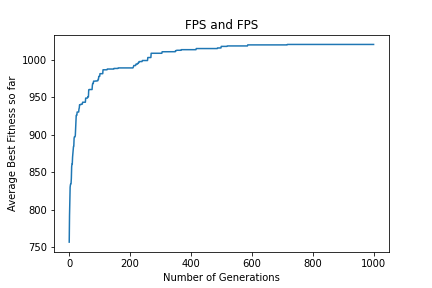
\includegraphics[width=12cm, height=7cm]{Graphs/KnapSack/fps_fps_bsf.png} \\
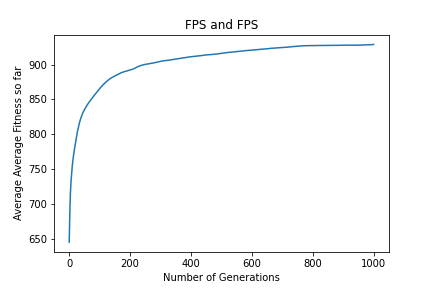
\includegraphics[width=12cm, height=7cm]{Graphs/KnapSack/fps_fps_avg.png} \\
\subsection{FPS and Random}
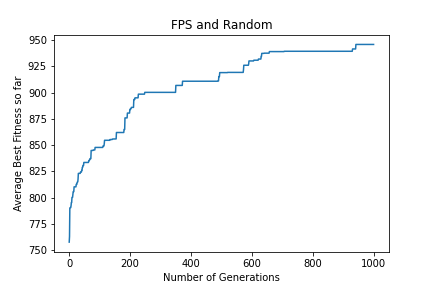
\includegraphics[width=12cm, height=7cm]{Graphs/KnapSack/fps_rand_bsf.png} \\
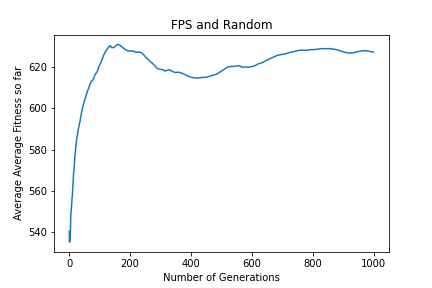
\includegraphics[width=12cm, height=7cm]{Graphs/KnapSack/fps_rand_avg.png} \\
\subsection{Binary Tournament and Truncation}
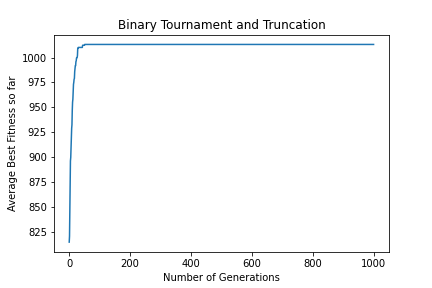
\includegraphics[width=12cm, height=7cm]{Graphs/KnapSack/bt_trunc_bsf.png} \\
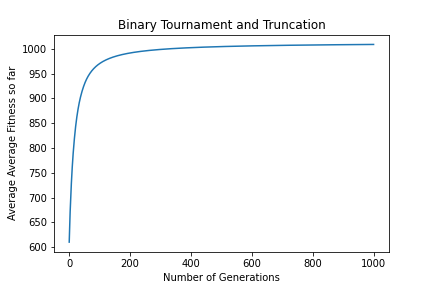
\includegraphics[width=12cm, height=7cm]{Graphs/KnapSack/bt_trunc_avg.png} \\
\subsection{Truncation and Truncation}
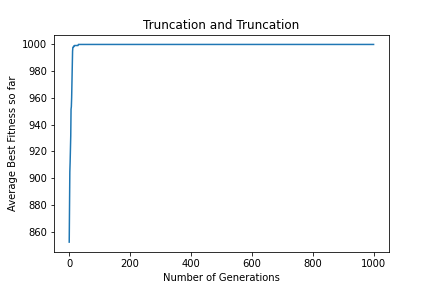
\includegraphics[width=12cm, height=7cm]{Graphs/KnapSack/trunc_trunc_bsf.png} \\
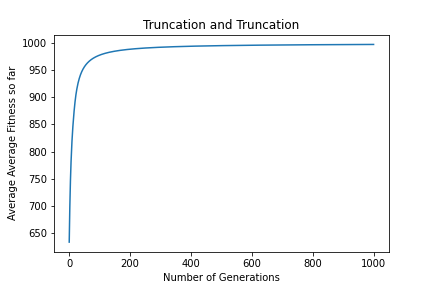
\includegraphics[width=12cm, height=7cm]{Graphs/KnapSack/trunc_trunc_avg.png} \\
\subsection{Random and Random}
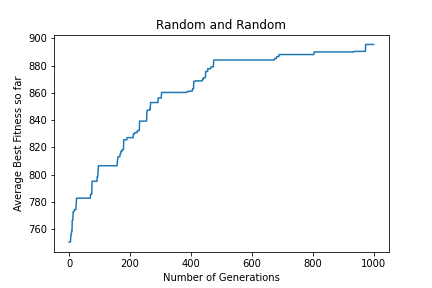
\includegraphics[width=12cm, height=7cm]{Graphs/KnapSack/rand_rand_bsf.png} \\
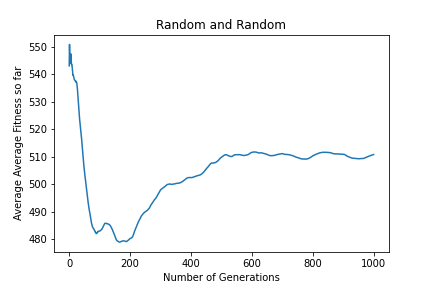
\includegraphics[width=12cm, height=7cm]{Graphs/KnapSack/rand_rand_avg.png} \\
\subsection{FPS and Truncation}
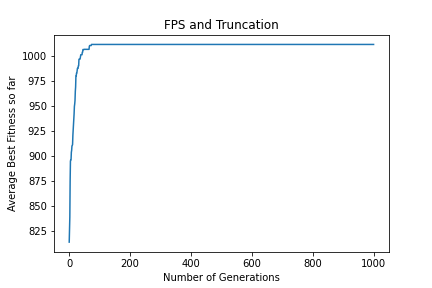
\includegraphics[width=12cm, height=7cm]{Graphs/KnapSack/fps_trunc_bsf.png} \\
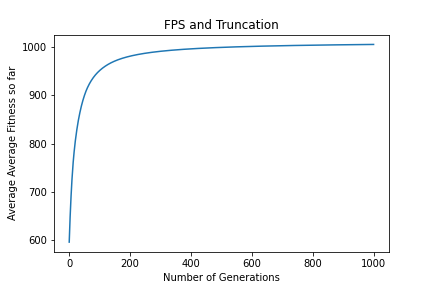
\includegraphics[width=12cm, height=7cm]{Graphs/KnapSack/fps_trunc_avg.png} \\
\subsection{RBS and Binary Tournament}
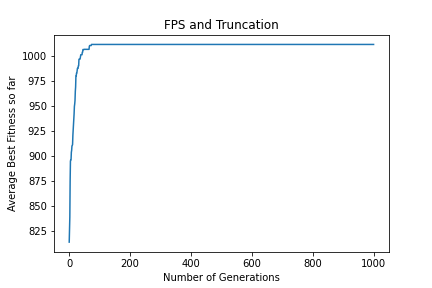
\includegraphics[width=12cm, height=7cm]{Graphs/KnapSack/fps_trunc_bsf.png} \\
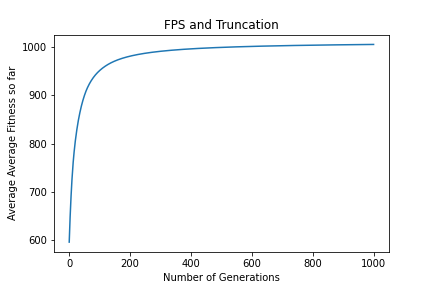
\includegraphics[width=12cm, height=7cm]{Graphs/KnapSack/fps_trunc_avg.png} \\
\subsection{Random and Truncation}
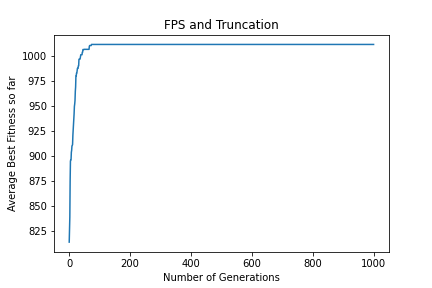
\includegraphics[width=12cm, height=7cm]{Graphs/KnapSack/fps_trunc_bsf.png} \\
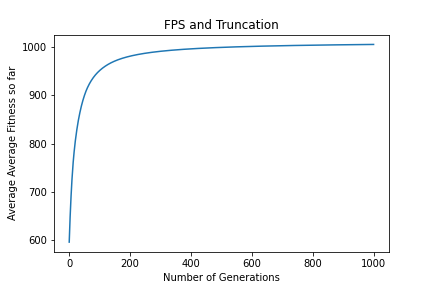
\includegraphics[width=12cm, height=7cm]{Graphs/KnapSack/fps_trunc_avg.png} \\


\section{Travelling Salesman}
The total number of cities was 194. The fitness of an individual chromosome was the reciprocal of the total distance covered with the start and end point being same. 
This is a minimisation optimisation problem, but we made it into a maximisation problem by taking the reciprocal.
\subsection{FPS and FPS}
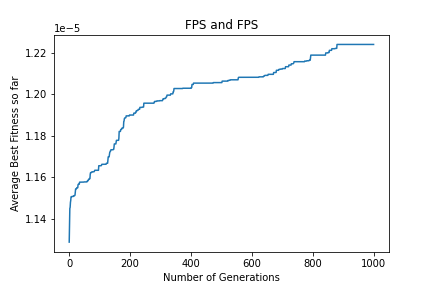
\includegraphics[width=12cm, height=7cm]{Graphs/TSP/fps_fps_bsf.png} \\
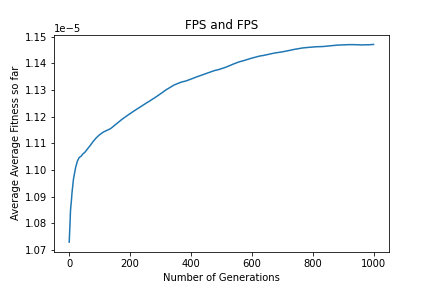
\includegraphics[width=12cm, height=7cm]{Graphs/TSP/fps_fps_avg.png} \\
\subsection{FPS and Random}
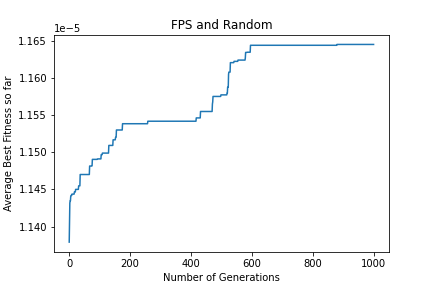
\includegraphics[width=12cm, height=7cm]{Graphs/TSP/fps_rand_bsf.png} \\
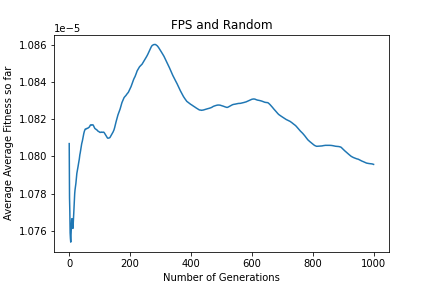
\includegraphics[width=12cm, height=7cm]{Graphs/TSP/fps_rand_avg.png} \\
\subsection{Binary Tournament and Truncation}
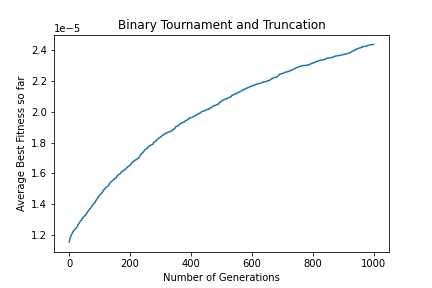
\includegraphics[width=12cm, height=7cm]{Graphs/TSP/bt_trunc_bsf.png} \\
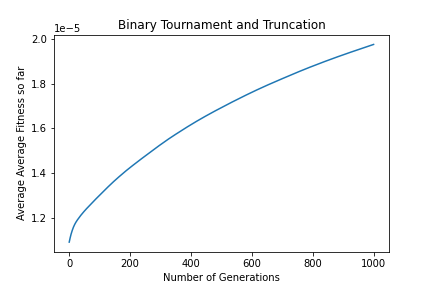
\includegraphics[width=12cm, height=7cm]{Graphs/TSP/bt_trunc_avg.png} \\
\subsection{Truncation and Truncation}
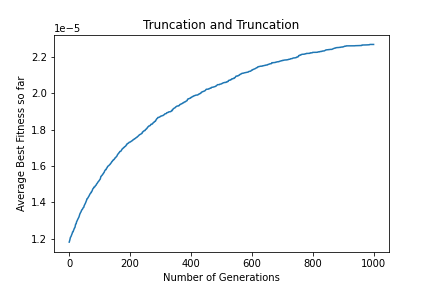
\includegraphics[width=12cm, height=7cm]{Graphs/TSP/trunc_trunc_bsf.png} \\
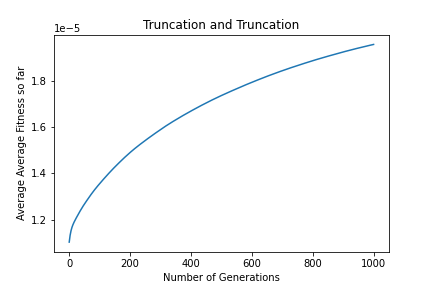
\includegraphics[width=12cm, height=7cm]{Graphs/TSP/trunc_trunc_avg.png} \\
\subsection{Random and Random}
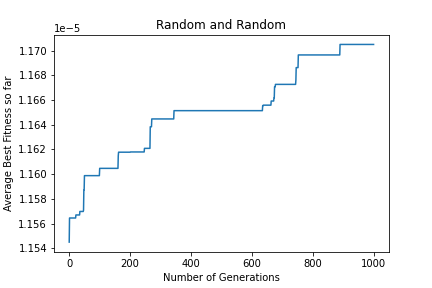
\includegraphics[width=12cm, height=7cm]{Graphs/TSP/rand_rand_bsf.png} \\
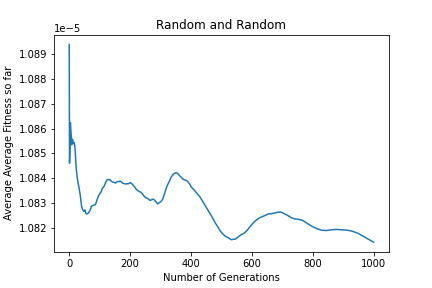
\includegraphics[width=12cm, height=7cm]{Graphs/TSP/rand_rand_avg.png} \\
\subsection{FPS and Truncation}
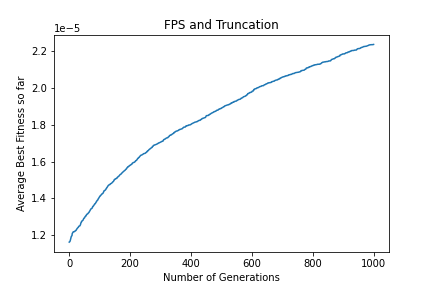
\includegraphics[width=12cm, height=7cm]{Graphs/TSP/fps_trunc_bsf.png} \\
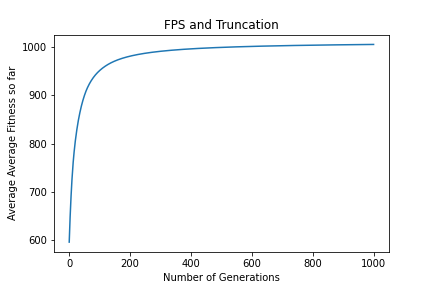
\includegraphics[width=12cm, height=7cm]{Graphs/KnapSack/fps_trunc_avg.png} \\
\subsection{RBS and Binary Tournament}
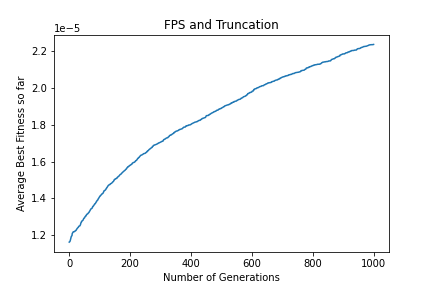
\includegraphics[width=12cm, height=7cm]{Graphs/TSP/fps_trunc_bsf.png} \\
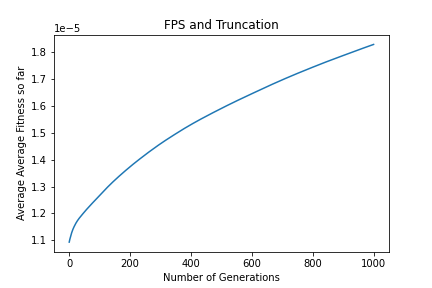
\includegraphics[width=12cm, height=7cm]{Graphs/TSP/fps_trunc_avg.png} \\
\subsection{Random and Truncation}
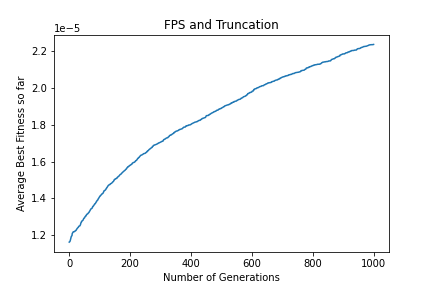
\includegraphics[width=12cm, height=7cm]{Graphs/TSP/fps_trunc_bsf.png} \\
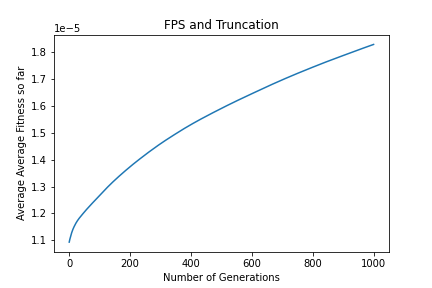
\includegraphics[width=12cm, height=7cm]{Graphs/TSP/fps_trunc_avg.png} \\

\section{Analysis \& Conclusion}

In case of the knapsack problem, apart from the combination of random select for the parents and survival scheme all the combinations produced acceptable results in a reasonable amount of time, and we achieved the optimum fitness of 1024 .  
This result was expected because Random Selection has a low selection pressure as compared to all other selection schemes.  Another reason was that the number of parameters was relatively low. Furthermore, due to smaller number of
parameters in the knapsack problem we did not need to tinker around with the parameters of the evolutionary algorithm.\newline

However, in the case of the travelling salesman problem, different combinations of rank-based selection, binary tournament, truncation and random selection excluding the combination of both parent and survivor scheme being random, produced acceptable results i.e. roundabout 20k, in a reasonable amount of the time.
This result was again expected because as the number of parameters that we required to optimise increase the complexity of the problem also increases. Moreover, the combination FPS and FPS did not produce convergence indicating the presence of some outliers. \newline

In order to achieve the optimal solution, we tinkered around with the values of the parameters of the evolutionary algorithm. Out of these, increasing the mutation rate to about 0.80 and the number of off springs to 20  increased the diversity which in turn caused the solution to converge.
We also seeded the population with some known candidate solutions instead of having a completely randomised population, but the results weren't entirely as expected. The average average fitness so far improved but the population didn't converge as much. \newline

The empirical results conformed with our expectations about how multiple schemes will work. As the number of parameters that are to be optimised, the complexity of the problem also increases greatly. Furthermore , in order to achieve an optimal solution , we need a combination of schemes that perform both exploitation and exploration. Another important factor that also needs to be considered before choosing different selections is the cost of computation.  
\end{document}